%************************************************
\chapter{Related Models}
\label{chapter:related_models}
%************************************************

The term reflection is a commonly used word in computer science and
AI.  The idea is extremely simple and is a modelling contribution of
this dissertation, but because of its simplicity, it is a widely
applicable idea.  In fact, \cite{maes:1987,maes:1988} distinguishes
over 30 different types of ``computational reflection,'' grounded in
the computer science literature.  The type of computational reflection
that is introduced in this dissertation is not included in Maes'
overview, although it is based on many of the forms of computational
reflection that Maes describes, i.e. procedural reflection, type
reflection, and frame reflection.

The SALS AI has been inspired by a previously implemented Emotion
Machine cognitive architecture called ``EM-ONE'' \cite[]{singh:2005b}.
EM-ONE implements reflective thinking using a commonsense narrative
representation based on an Allegro Prolog extension of Allegro Lisp.
The EM-ONE architecture is a ``critic-selector'' model of problem
solving
\cite[]{sussman:1973,singh:2002a,singh:2004,singh:2005a,singh:2005b,minsky:2006,morgan:2009}.
Knowledge in the EM-ONE architecture is divided into three domains:
(1) physical, (2) social, and (3) mental.  The EM-ONE AI controls a
physical simulation that contains two one-armed robots that can work
together to build a table.  The EM-ONE AI contains three layers of
reflective control: (1) reactive, (2) deliberative, and (3)
reflective.  While the EM-ONE cognitive architecture represents the
first major implementation of the Emotion Machine theory of mind, it
was limited in a number of ways:
\begin{packed_enumerate}
\item{Critics are specified in a declarative logical form, which does
  not allow for learning to optimize the procedural aspects of
  Prolog's implicit declarative search.}
\item{The implemented ``Critic-L'' language allows for inserted
  procedural Lisp code, but any procedural code inserted in this way
  is not reflectively traced.}
\item{Only learns from ``being told'' commonsense narratives and does
  not learn from its ``experience'' in order to better predict the
  effects of executing its physical or mental actions.}
\item{Commonsense narratives cannot be specified in natural language.}
\item{All activities execute in serial, so no critics or selectors can
  execute in parallel.  Reasoning activities in each layer also occur
  in serial, so that the layers of control cannot execute
  concurrently.}
\item{Does not take advantage of multiple CPUs or CPUs with multiple
  cores.}
\item{Allegro Lisp and Allegro Prolog are expensive tools, barring
  collaborative research with many independent researchers that cannot
  afford such tools.}
\end{packed_enumerate}
The SALS cognitive architecture aims to provide one cohesive solution
to these limitations in the foundation of the EM-ONE Emotion Machine
implementation.  In focusing on solving these limitations, the SALS
architecture has failed to model some good aspects of the EM-ONE
architecture.  The following are a number of parts of EM-ONE that are
still future research for the SALS AI:
\begin{packed_enumerate}
\item{Self-reflective social knowledge.}
\item{The ability to refer to arbitrary partial states of a problem
  domain.}
\item{Critics.}
\end{packed_enumerate}
The EM-ONE architecture includes a separate knowledge base for storing
self-reflective social knowledge, the knowledge in the minds of other
AIs, such as their beliefs and goals.  The ability of an AI to learn
abstract models of its own mind and use these models to hypothesize
the state of mind in other AIs is referred to as ``self-reflective''
thinking in the Emotion Machine theory.  This type of self-reflective
thinking is also referred to as ``theory of mind'' in the cognitive
science literature and has been found to exist in different neural
circuits in the brain when compared to deliberative or ``executive''
functions in the brain \cite[]{saxe:2006}.  Because the EM-ONE
architecture is based on a Prolog substrate, it has the ability to
refer to arbitrary partial states of a problem domain, while the SALS
AI is currently limited to the two simple ``relationship'' and
``property'' types of partial states, which must be procedurally
combined in order to reference more complex types of partial states.
This means that the EM-ONE architecture can easily define critics that
recognize arbitrarily complex declarative patterns in the problem
domain.  The disadvantage of relying on a declarative substrate, such
as Prolog, is that the procedural aspects of this substrate are not
reflectively traced and cannot be optimized by the EM-ONE
architecture.  While the SALS architecture must have explicit plans
for recognizing more complex partial states, the fact that these
procedures are plans in the SALS AI means that different procedures
for recognizing these partial states in the problem domain can be
reflected upon, modified, compared and optimized by the SALS AI.  The
addition of critics as well as self-reflective and self-conscious
layers of thinking is described as a future extension for the SALS
architecture in {\mbox{\autoref{chapter:future}}}.

\section{Computational Metacognition}

The type of reflection implemented in this thesis is a form of
``computational metacognition'' \cite[]{cox_and_raja:2008,cox:2010}:
the ability to think about accomplishing thinking goals in addition to
thinking about accomplishing physical goals.  Computational
metacognition as described by Cox and Raja begins with a ``ground
level,'' which is the problem domain for the AI to control.  The
computational metacognition ground level is analogous to the physical
knowledge base and physical agency of the learned reactive layer in
the SALS Emotion Machine cognitive architecture.  The ``object level''
of computational metacognition is a control loop that receives inputs
from the ground level, processes these, and sends commands back to the
ground level.  The object level of computational metacognition is
analogous to the deliberative planning layer in the SALS Emotion
Machine cognitive architecture.  The ``meta-level'' of computational
metacognition completes two cascaded control loops: the object level
controlling the ground level and the meta-level controlling the object
level.  The meta-level of computational metacognition is analogous to
the reflective planning layer of the SALS Emotion Machine cognitive
architecture.
\begin{table}
\begin{tabular}{|rll|}
\hline
Metacognition Meta Level   &${\approx}$ &Emotion Machine Reflective Layer \\
Metacognition Object Level &${\approx}$ &Emotion Machine Deliberative Layer \\
Metacognition Ground Level &${\approx}$ &Emotion Machine Learned Reactive Layer \\
\hline
\end{tabular}
\caption{The levels of computational metacognition mapped to the
  Emotion Machine cognitive architecture presented in this
  dissertation.}
\label{table:computational_metacognition_as_reflective_order_notation}
\end{table}
\autoref{table:computational_metacognition_as_reflective_order_notation}
shows how the levels of computational metacognition map to the Emotion
Machine cognitive architecture presented in this dissertation.

\section{Meta-planning and Meta-Plan Recognition}

\cite{wilensky:1981} describes ``meta-planning'' as representing and
using knowledge about planning in problem solving and natural language
understanding domains.  He describes ``PAM,'' a story understanding
system, and ``PANDORA,'' a story understanding and problem solving
system, that both use higher-level goals and plans that he calls
``meta-goals'' and ``meta-plans.''  The basic goals and plans in
PANDORA are analogous to the goals and plans in the SALS deliberative
planning layer, while the meta-goals and meta-plans are analogous to
the goals and plans in the SALS reflective planning layer.  Wilensky
describes story understanding as a form of inverse planning or plan
recognition.  In this sense, a planning system is given a set of goals
that are used to generate a sequence of actions that accomplish the
goals, while a story understanding system is given a sequence of
actions that are used to generate a set of goals that explain those
actions.  Wilensky emphasizes that both story understanding and
planning require representations of meta-goals and meta-plans in order
to reason about common types of human thinking.  Wilensky gives the
following two example story understanding problems:
\begin{packed_enumerate}
\item{John was in a hurry to get to Las Vegas, but he noticed that
  there were a lot of cops around so he stuck to the speed limit.}
\item{John was eating dinner when he noticed that a thief was trying
  to break into his house.  After he finished his dessert, John called
  the police.}
\end{packed_enumerate}
In Wilensky's first example, John is understood to have two goals: (1)
to get to Las Vegas as quickly as possible, and (2) to avoid getting a
ticket.  Wilensky's reasoning system recognizes that these two goals
conflict and that John has pursued the meta-goal of resolving goal
conflicts.  Because getting a ticket has more negative value than the
positive value of getting to Las Vegas quickly, it understands that
the goal of speeding is abandoned due to pursuing this meta-goal.  In
the second story, Wilensky's reasoning system recognizes that John has
made an unintelligent decision to continue eating his dessert while
someone is robbing his house.  In terms of meta-goals, Wilensky's
system recognizes that John did not have the meta-goal to delay
pursuing a less valuable goal in light of the presence of a new more
valuable goal.  So, Wilensky's system is able to perform meta-planning
and meta-plan recognition, which are both future research goals for
the SALS architecture.  There are a few key differences between the
SALS architecture and PANDORA:
\begin{packed_enumerate}
\item{Meta-goals and goals in PANDORA are considered the same type of
  knowledge and are stored in the same knowledge base that is reasoned
  about by one monolithic planner, while the SALS AI keeps these
  categorically different types of knowledge separated into
  hierarchical layers of different knowledge bases and types of
  planning processes.}
\item{Because PANDORA is not connected to an external problem domain,
  while the SALS AI responds to the various types of plan failures
  that result from executing plans, such as physical expectation
  failures.}
\item{PANDORA only learns from ``being told'' knowledge, while the
  SALS AI learns from both ``being told'' natural language plans as
  well as from the ``experience'' of executing these plans.}
\end{packed_enumerate}

%\section{Meta-AQUA Story Understanding}



%% \section{Meta-management}

%% Varieties of Meta-cognition in Natural and Artificial Systems
%% \cite[]{sloman:2011}.

%% \begin{quote}
%% One implication of the generalisation to biological phenomena (and
%% human-like robots) is that the ``ground level'' ... may include
%% arbitrarily complex physical and social environments.  In humans,
%% while awake, there are sensors and effectors continuously coupled to
%% the environment: i.e. the coupling does not alternate between being on
%% and off while more central processes analyze sensory inputs or decide
%% what to do. Consequently, instead of an ``action-perception cycle,''
%% we need an architecture with concurrent processes of many kinds, which
%% can interact with one another. (Even a single-cpu computer can support
%% concurrent enduring processes because, while the cpu is shared, the
%% majority of the state of each process endures in memory.
%% \end{quote}

%% \section{Massively Multithreaded Programming}

%% Optimization principles and application performance evaluation of a
%% multithreaded GPU using CUDA \cite[]{ryoo:2008}.







\section{Optimality in Metacognition}

AI researchers often approach problem solving from the perspective of
theories of ``rationality'' from the fields of decision theory and
economics.  From this perspective, rationality requires the AI to
decide upon optimal actions with respect to the values or costs of its
goals and activities.  In the basic formulation, different actions
have different costs and the optimal decision is the decision that
minimizes this cost over some time period, possibly an infinite
horizon.  In simple domains, the solution to a problem of optimal
control can be specified in closed form \cite[]{bertsekas:1995}.  In
complex domains, optimal decision making requires intractable
computations to be performed, and approximate or ``satisficing''
solutions to problems become necessary \cite[]{simon:1957,simon:1982}.
\cite{good:1971} describes a decision making problem that includes
costs for acting as well as costs for decision making that he calls
``type II rationality,'' a type of metacognition.
\cite{zilberstein:2008} describes ``optimal metareasoning'' as an
approach to developing a formalism for evaluating the performance of a
problem solver that is performing type II rationality.  Optimal
metacognition does not imply that the object level problem solver is
optimal but instead that the meta-level problem solver is optimal.  In
``bounded optimality'' the object level problem solver has certain
trade-offs, such as solution quality versus time, that can be
optimally manipulated by the meta-level problem solver
\cite[]{russell:1991}.  \cite{zilberstein:2008} describes bounded
optimality:
\begin{quote}
This approach marks a shift from optimization over actions to
optimization over programs.  The program is bounded optimal for a
given computational device for a given environment, if the expected
utility of the program running on the device in the environment is at
least as high as that of all other programs for the device.  When the
space of programs is finite, one can certainly argue that a bounded
optimal solution exists.  Finding it, however, could be very hard.
\end{quote}
While the SALS AI is neither an optimal problem solver nor an optimal
meta-level problem solver, the field of optimal problem solving does
have the attractive feature that there is an objective metric of
performance for all problem solving algorithms when viewed through the
lens of optimality.  There are a few key differences between most
optimal meta-planning algorithms and the SALS AI:
\begin{packed_enumerate}
\item{Optimal metacognitive algorithms only learn from ``experience,''
  while the SALS AI learns both from ``being told'' natural language
  plans as well as from the ``experience'' of executing these plans.}
\item{Optimal metacognitive algorithms tend to only consider simple
  control parameters of an object-level algorithm, such as the
  allocated execution time for a contract or anytime algorithm, while
  the SALS AI considers all possible programs that implement
  object-level reasoning.}
\end{packed_enumerate}
While the SALS AI does not currently have an objective performance
metric, it is interesting to consider how the field of bounded
rationality could benefit from ``being told'' deliberative and
reflective natural language plans as a method of more quickly
searching the space of all possible planning programs.

%% \cite{horvitz:1988} describes bounded rationality as 
%% The bounded optimality approach to metacognition is primarily focused
%% on allocating computational resources to improve the ground
%% performance of the object level algorithm in the problem domain.  If
%% the object level problem solving algorithm is specified as an
%% ``anytime'' algorithm, meaning that .



%% \section{Interior Grounding}

%% \cite{minsky:2005} describes an evolutionary reflective model of mind
%% called ``interior grounding.''  Interior grounding states that each
%% layer of reflective thinking could be genetically predestined to each
%% have different and specific types of useful ways of thinking.  Minsky
%% rejects the ``physical grounding hypothesis,'' which stipulates that
%% thoughts must necessarily develop from the lowest layer first and only
%% subsequently to the higher layers of thinking.

%% Because my AI is modelled after Minsky's Emotion Machine cognitive
%% architecture, activities in the mind can create and manipulate
%% symbolic arrangements without these symbols necessarily referring to
%% the physical layer of activity.  My model considers factual grounding
%% in both the perception of physical knowledge as well as the perception
%% of internal mental states, such as the deliberative planning machine
%% knowledge.

%% In terms of the Emotion Machine cognitive architecture, each
%% reflective layer of my model can be considered to have a unique
%% built-in reactive layer, which makes room for these genetic
%% dispositions that Minsky describes as the basis for interior
%% grounding.  My AI demonstrates interior grounding by having sets of
%% factual knowledge as the control domain for both the deliberative as
%% well as the reflective planning machines, so factual grounding of
%% hypothetical counterfactual inferences in my AI need not begin by
%% reasoning about physical activity, growing from lower layers to higher
%% layers, but may instead begin by reasoning about the factual events in
%% the deliberative planning machine knowledge bases.

%% \section{HACKER}

%% A good precedent for reflective debugging responses to catalogs of
%% failures is ``HACKER,'' one of the first reflective planning and
%% debugging models, written by \cite{sussman:1973}.  [complete]

%% \section{Propagators}

%% \cite{radul_and_sussman:2009} describe an object called a \emph{cell}
%% that is closely related to the knowledge dependencies depicted in
%% {\mbox{\autoref{figure:dependency_traces}}}.  These cells can be
%% connected by dependency sets that specify functions that derive new
%% knowledge from the dependencies, as well as, functions for merging the
%% collected knowledge in cells.  Collections of Radul and Sussman's
%% cells are called a \emph{propagator}.  The knowledge dependencies in
%% this model can be thought of as a type of propagator.  The combination
%% of a propagator model of knowledge maintenance with a reflective
%% organization is described as future research in
%% \autoref{chapter:future}.
%% %\begin{figure}
%% %\center
%% %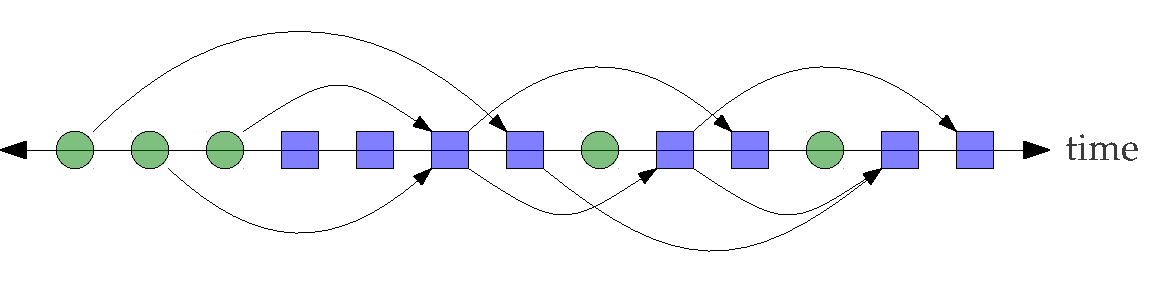
\includegraphics[width=10cm]{gfx/dependency_traces}
%% %\caption{Dependency traces as propagator cells.}
%% %\label{figure:propogators_dependency_traces}
%% %\end{figure}

